\section{Конструкторский раздел \hfill}
\vspace{\baselineskip}

В данном разделе будут приведены схемы алгоритмов поиска расстояний Левенштейна и Дамерау-Левенштейна. При разработке этих алгоритмов можно использовать разные подходы к реализации: итеративный, рекурсивный без кеширования, рекурсивный с кешированием.

\subsection{Алгоритм поиска расстояния Левенштейна}

На рисунке \ref{fig:l-matr} приведена схема нерекурсивного алгоритма поиска расстояния Левенштейна с заполнением матрицы расстояний.

\newpage
\begin{figure}[h!btp]
    \captionsetup{justification=centering}
	\centering
	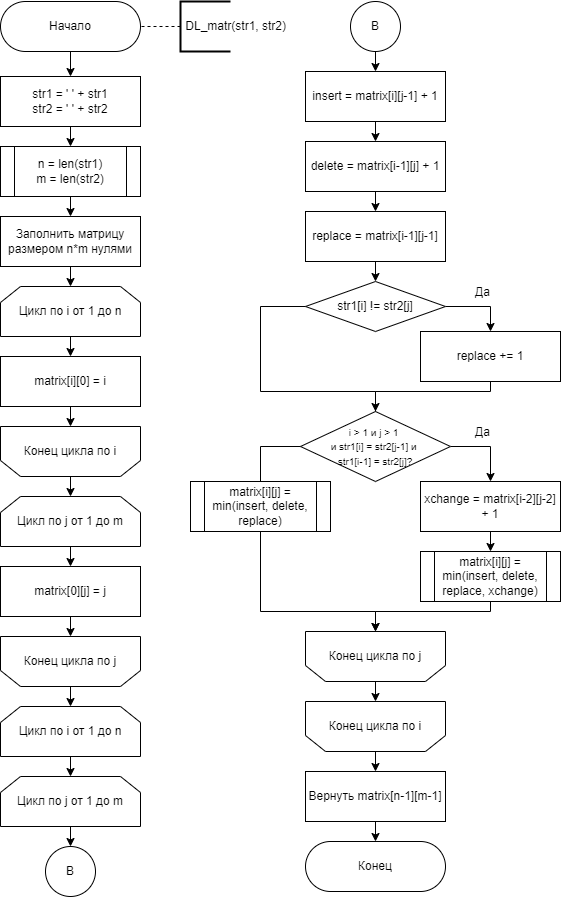
\includegraphics[width=360pt]{inc/dl-matr.png}
	\caption{Схема нерекурсивного алгоритма поиска расстояния Левенштейна}
	\label{fig:l-matr}	
\end{figure}
\clearpage

\subsection{Алгоритмы поиска расстояния Дамерау-Левенштейна}

На рисунках \ref{fig:dl-matr}, \ref{fig:dl-rec}, \ref{fig:dl-rec-opt} приведены схемы следующих алгоритмов:

\begin{itemize}
    \item итеративного алгоритма поиска расстояния Дамерау-Левенштейна с заполнением матрицы расстояний;
    \item рекурсивного алгоритма поиска расстояния Дамерау-Левенштейна без кеширования;
    \item рекурсивного алгоритма поиска расстояния Дамерау-Левенштейна с кешированием.
\end{itemize}
\clearpage

\begin{figure}[h!btp]
    \captionsetup{justification=centering}
	\centering
	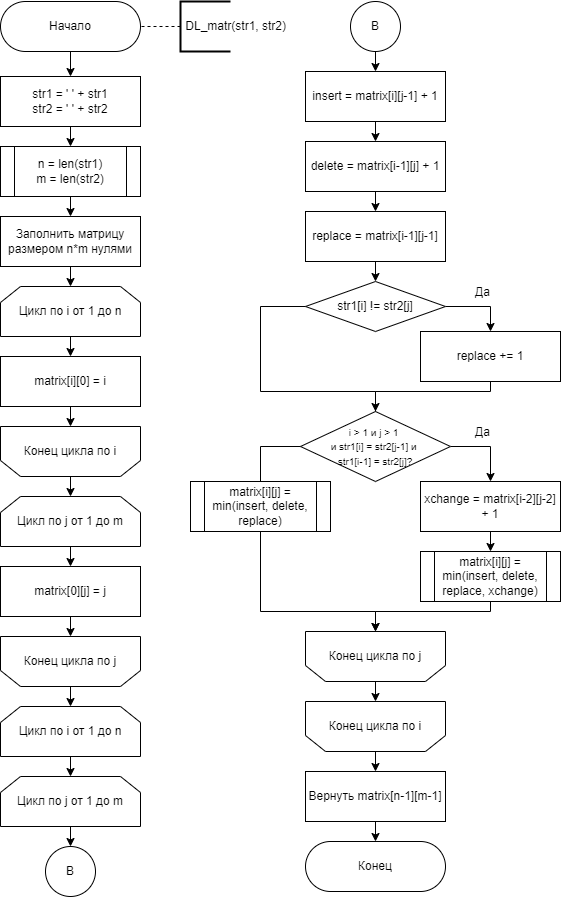
\includegraphics[width=380pt]{inc/dl-matr.png}
	\caption{Схема нерекурсивного алгоритма поиска расстояния Дамерау-Левенштейна}
	\label{fig:dl-matr}	
\end{figure}
\clearpage

\begin{figure}[h!btp]
    \captionsetup{justification=centering}
	\centering
	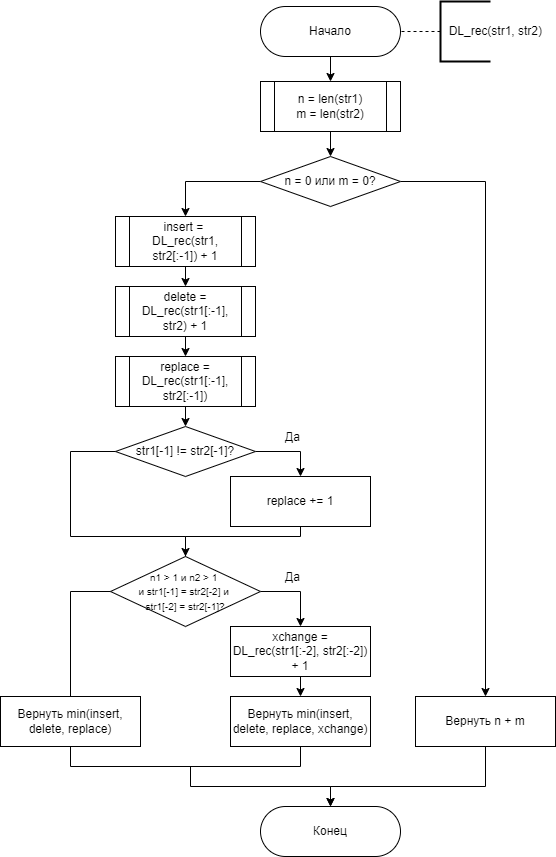
\includegraphics[width=380pt]{inc/dl-rec.png}
	\caption{Схема рекурсивного алгоритма поиска расстояния Дамерау-Левенштейна без кеширования}
	\label{fig:dl-rec}	
\end{figure}
\clearpage

\begin{figure}[h!btp]
    \captionsetup{justification=centering}
	\centering
	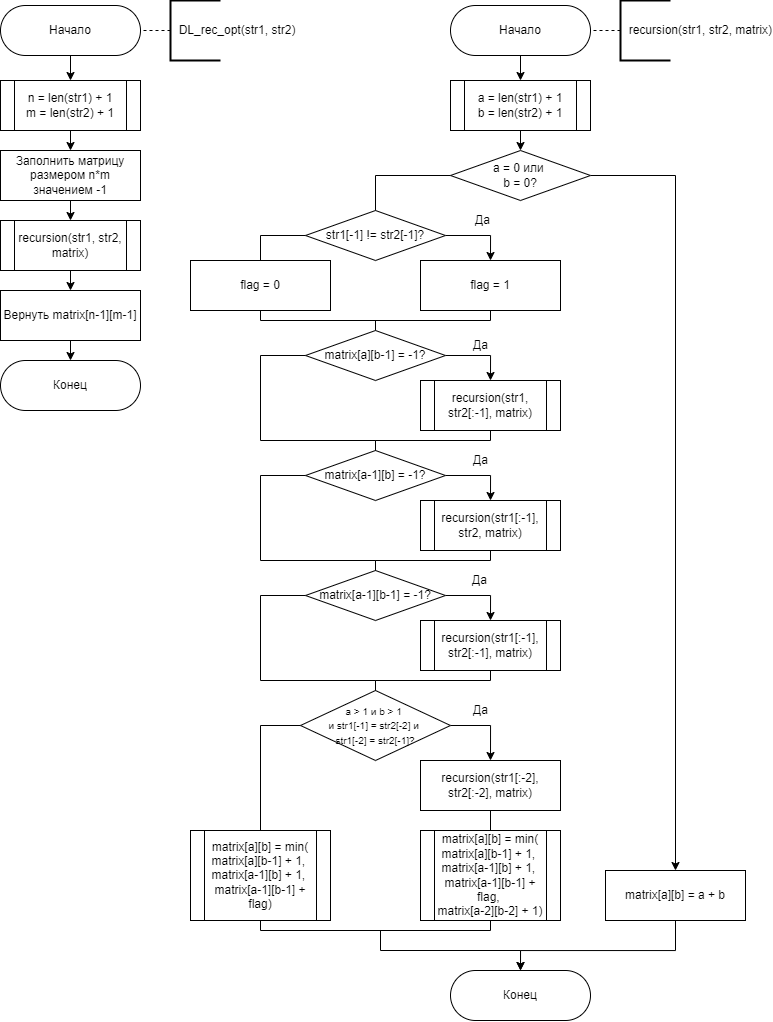
\includegraphics[width=450pt]{inc/dl-rec-opt.png}
	\caption{Схема рекурсивного алгоритма поиска расстояния Дамерау-Левенштейна с кешированием}
	\label{fig:dl-rec-opt}	
\end{figure}
\clearpage


\subsection*{Вывод}

Были разработаны схемы алгоритмов, позволяющих находить расстояния Левенштейна и Дамерау-Левенштейна. 